% begin module first-derivative-test
\begin{frame}
\begin{itemize}
\item  Recall that if $f$ has a local maximum at $c$, then $c$ must be a critical number for $f$, but if $c$ is a critical number for $f$, it is not necessarily a local maximum.
\item<2->  In the first picture, \alert<2>{$f'(x) > 0$ to the left of $c$} and \alert<2>{$f'(x) < 0$ to the right} of $c$.
\item<3->  In other words, $f'(x)$ changes sign at $c$.
\item<4->  In the second picture, \alert<4>{$f'(x) > 0$ to the left} of $c$ and \alert<4>{$f'(x) > 0$ to the right} of $c$.  $f'(x)$ doesn't change sign at $c$.
\item<5->  In the first picture there's a local maximum, but not in the second.
\item<6->  This suggests a way of testing for local maxima/minima.
\end{itemize}
\begin{columns}[c]
\column{.5\textwidth}
\psset{xunit=1.2cm, yunit=1.2cm}
\begin{pspicture}(-5, -5)(5,5) 
\psframe*[linecolor=white](-5,-5)(5,5) 
\tiny
\psaxes[ticks=none, labels=none]{<->}(0,0)(-0.5,-0.5)(3.3,2.6)
\psLabels{3.3}{2.6}
%Function formula: -5/2-2 ((x) (x))+6 (x) 
\psplot[linecolor=red, plotpoints=1000]{0.39}{2.61}{x 6 mul x x mul -2 mul add -2.5 add }
%Function formula: -2 (x)+11/2 
\psplot[linecolor=\psColorTangent, plotpoints=1000]{1.7}{2.3}{5.5 x -2 mul add } %Function formula: 2 (x)-1/2 
\psplot[linecolor=\psColorTangent, plotpoints=1000]{0.7}{1.3}{-0.5 x 2 mul add } 
\psline[linecolor=\psColorTangent](1.3,2)(1.7,2)
\psline[linestyle=dashed](1.5, 2)(1.5, 0)
\tiny
\rput[t](1.5, -0.1){$c$}
\rput[l](0.1, 1.6) {\alert<2>{$f'(x)>0$}}
\rput[r](2.9, 1.6) {\alert<2>{$f'(x)<0$}}
\end{pspicture} 

%\ %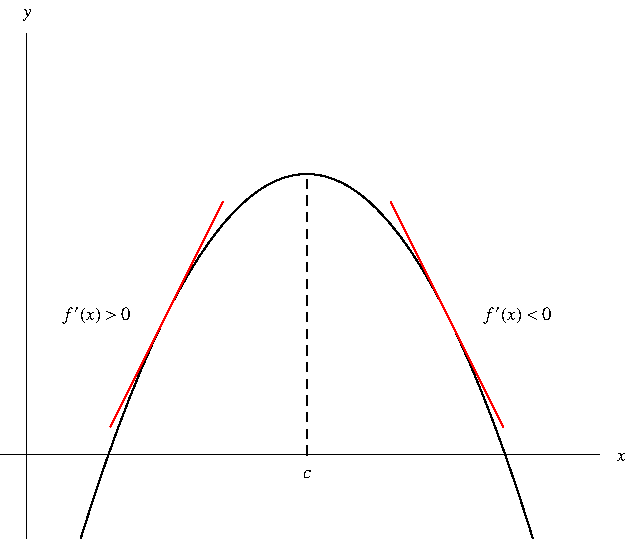
\includegraphics[height=3cm]{curve-sketching/pictures/04-03-firstderiva.pdf}%
\column{.5\textwidth}
\psset{xunit=1.2cm, yunit=1.2cm}
\begin{pspicture}(-0.5, -5)(2.9,5) 
\psframe*[linecolor=white](-0.5,-5)(2.9,5) 
\tiny 
\psaxes[ticks=none, labels=none]{<->}(0,0)(-0.5,-0.5)(3.3,2.6)
\psLabels{3.3}{2.6}
%Function formula: (-17/10+x)^{3}+1/2 
\psplot[linecolor=\psColorGraph, plotpoints=1000] {0.73} {2.9} {0.5 x -1.7 add 3 exp add }
%\psFullDot{1}{0.157}
%\psFullDot{2.4}{0.843}
%Function formula: -1313/1000+147/100 (x) 
\psplot[linecolor=\psColorTangent, plotpoints=1000] {0.65} {1.35} {x 1.47 mul -1.313 add }
%Function formula: -537/200+147/100 (x) 
\psplot[linecolor=\psColorTangent, plotpoints=1000] {2.05} {2.75} {x 1.47 mul -2.685 add }
\psline[linecolor=\psColorTangent](1.35,0.492)(2.05,0.492)
\psline[linestyle=dashed](1.7, 0)(1.7, 0.492)
\rput[t](1.7, -0.1){$c$}
\rput(0.5,0.6){\alert<4>{$f'(x)>0$}}
\rput(2.8,0.6){\alert<4>{$f'(x)>0$}}
\end{pspicture} 

%\ %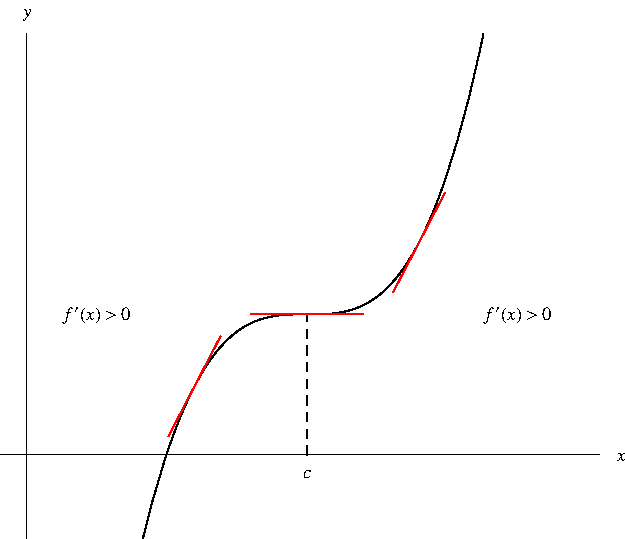
\includegraphics[height=3cm]{curve-sketching/pictures/04-03-firstderivc.pdf}%
\end{columns}
\end{frame}



\begin{frame}
The First Derivative Test

Suppose that $c$ is a critical number of a continuous function $f$.
\begin{enumerate}
\item<1-| alert@2>  \alert<handout:1| 0>{If $f'$ changes from positive to negative at $c$, then $f$ has a local maximum at $c$.}
\item<1-| alert@3>  \alert<handout:2| 0>{If $f'$ changes from negative to positive at $c$, then $f$ has a local minimum at $c$.}
\item<1-| alert@4>  \alert<handout:3| 0>{If $f'$ doesn't change signs at $c$, then $f$ has no local maximum or minimum at $c$.}
\end{enumerate}
\begin{columns}[c]
\column{.5\textwidth}
\psset{xunit=1.2cm, yunit=1.2cm}
\begin{pspicture}(-5, -5)(5,5) 
\psframe*[linecolor=white](-5,-5)(5,5) 
\tiny
\psaxes[ticks=none, labels=none]{<->}(0,0)(-0.5,-0.5)(3.3,2.6)
\psLabels{3.3}{2.6}
%Function formula: -5/2-2 ((x) (x))+6 (x) 
\uncover<2>{
\psplot[linecolor=red, plotpoints=1000]{0.39}{2.61}{x 6 mul x x mul -2 mul add -2.5 add }
%Function formula: -2 (x)+11/2 
\psplot[linecolor=\psColorTangent, plotpoints=1000]{1.7}{2.3}{5.5 x -2 mul add } %Function formula: 2 (x)-1/2 
\psplot[linecolor=\psColorTangent, plotpoints=1000]{0.7}{1.3}{-0.5 x 2 mul add } 
\psline[linestyle=dashed](1.5, 2)(1.5, 0)
\tiny
\rput[t](1.5, -0.1){$c$}
\rput[l](0.1, 1.6) {\alert<2>{$f'(x)>0$}}
\rput[r](2.9, 1.6) {\alert<2>{$f'(x)<0$}}
}
\uncover<3>{
%Function formula: 1/2+2 ((-3/2+x)^{2}) 
\psplot[linecolor=\psColorGraph, plotpoints=1000]{0.5}{2.5}{x -1.5 add 2 exp 2 mul 0.5 add }
%Function formula: -3+2 (x) 
\psplot[linecolor=\psColorTangent, plotpoints=1000]{1.7}{2.3}{x 2 mul -3 add }
%Function formula: 3-2 (x) 
\psplot[linecolor=\psColorTangent, plotpoints=1000]{0.7}{1.3}{x -2 mul 3 add }
\psline[linestyle=dashed](1.5, 0.5)(1.5, 0)
\tiny
\rput[t](1.5, -0.1){$c$}
\rput[l](0.1, 0.8) {\alert<3>{$f'(x)<0$}}
\rput[r](2.9, 0.8) {\alert<3>{$f'(x)>0$}}
}
\uncover<4->{
%Function formula: (-17/10+x)^{3}+1/2 
\psplot[linecolor=\psColorGraph, plotpoints=1000] {0.73} {2.9} {0.5 x -1.7 add 3 exp add }
%\psFullDot{1}{0.157}
%\psFullDot{2.4}{0.843}
%Function formula: -1313/1000+147/100 (x) 
\psplot[linecolor=\psColorTangent, plotpoints=1000] {0.65} {1.35} {x 1.47 mul -1.313 add }
%Function formula: -537/200+147/100 (x) 
\psplot[linecolor=\psColorTangent, plotpoints=1000] {2.05} {2.75} {x 1.47 mul -2.685 add }
\psline[linecolor=\psColorTangent](1.35,0.492)(2.05,0.492)
\psline[linestyle=dashed](1.7, 0)(1.7, 0.492)
\rput[t](1.7, -0.1){$c$}
\rput(0.5,0.6){\alert<4>{$f'(x)>0$}}
\rput(2.8,0.6){\alert<4>{$f'(x)>0$}}
}
\end{pspicture} 

%\ \only<handout:1| -2>{%
%\uncover<2>{%
%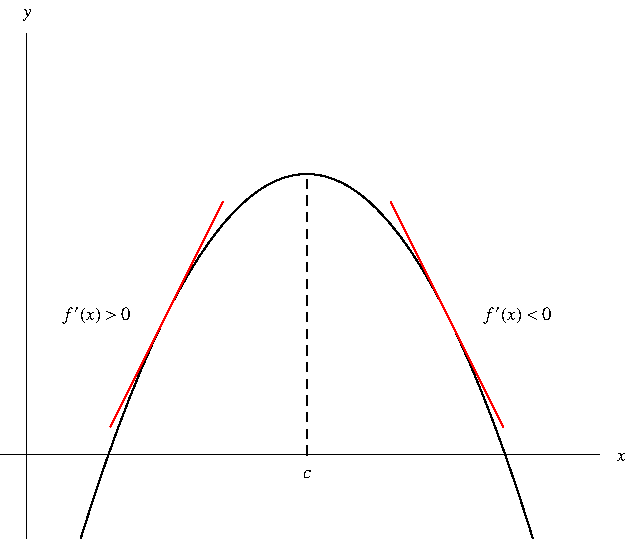
\includegraphics[height=4cm]{curve-sketching/pictures/04-03-firstderiva.pdf}%
%}
%}%
%\only<handout:2| 3>{%
%\uncover<3>{%
%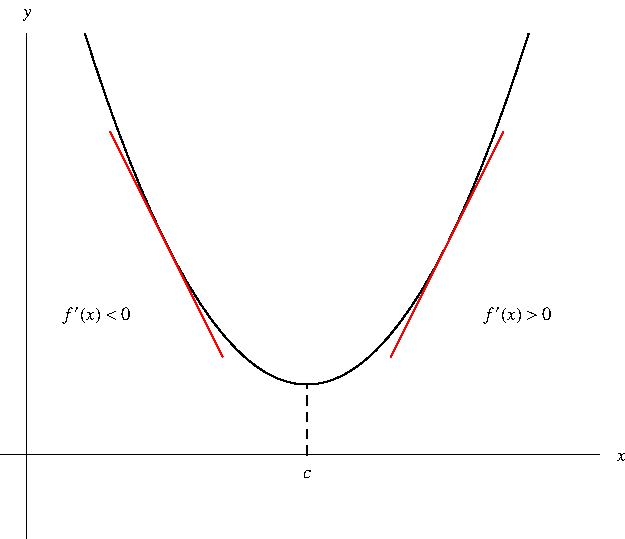
\includegraphics[height=4cm]{curve-sketching/pictures/04-03-firstderivb.pdf}%
%}}%
%\only<handout:3| 4->{%
%\uncover<4->{%
%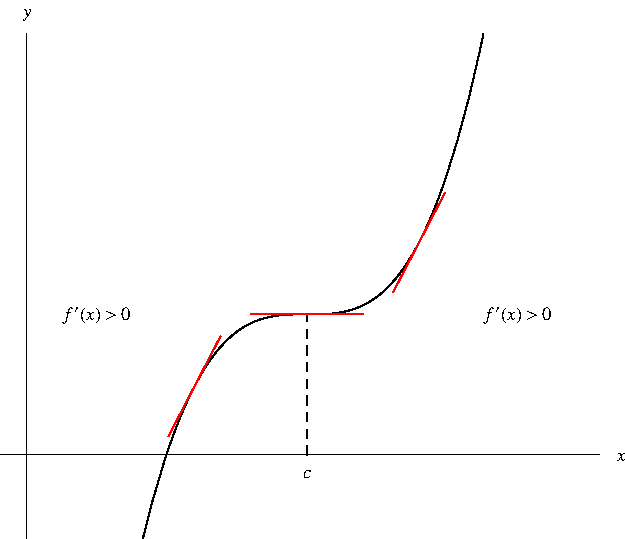
\includegraphics[height=4cm]{curve-sketching/pictures/04-03-firstderivc.pdf}%
%} }%
\column{.5\textwidth}
\psset{xunit=1.2cm, yunit=1.2cm}
\begin{pspicture}(-0.5, -5)(2.9,5) 
\psframe*[linecolor=white](-0.5,-5)(2.9,5) 
\tiny 
\psaxes[ticks=none, labels=none]{<->}(0,0)(-0.5,-0.5)(3.3,2.6)
\psLabels{3.3}{2.6}
\uncover<4>{
%Function formula: 1/2- ((-17/10+x)^{3}) 
\psplot[linecolor=\psColorGraph, plotpoints=1000]{0.5}{2.65}{x -1.7 add 3 exp -1 mul 0.5 add }
%Function formula: 737/200-147/100 (x) 
\psplot[linecolor=\psColorTangent, plotpoints=1000]{2.1}{2.7}{x -1.47 mul 3.685 add }
%Function formula: 2313/1000-147/100 (x) 
\psplot[linecolor=\psColorTangent, plotpoints=1000]{0.7}{1.3}{x -1.47 mul 2.313 add }
\psline[linecolor=\psColorTangent](1.35,0.492)(2.05,0.492)
\psline[linestyle=dashed](1.7, 0)(1.7, 0.5)
\rput[t](1.7, -0.1){$c$}
\rput(0.5,0.6){\alert<4>{$f'(x)<0$}}
\rput(2.8,0.6){\alert<4>{$f'(x)<0$}}
}
\end{pspicture} 
%\uncover<handout:3| 4->{%
%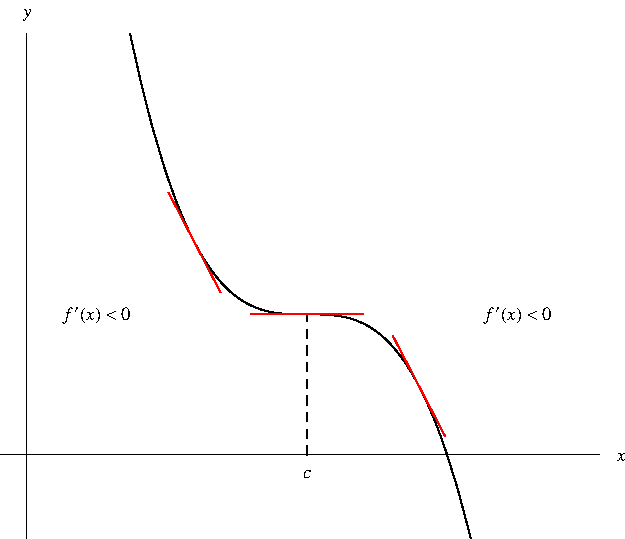
\includegraphics[height=4cm]{curve-sketching/pictures/04-03-firstderivd.pdf}%
%}%
\end{columns}
\end{frame}
% end module first-derivative-test
